\documentclass{beamer}

\usepackage{afit-beamer-template}
\graphicspath{{diagrams/},{figure/},{afit-images/}} 

\usepackage{booktabs}

% Command line/terminal-like environment
% Todo tag
\newcommand{\tbd}[1]{{\color{red} TBD: #1}}



\title[Title Desert]{Malicious Traffic Detection through Internet Protocol Address Hopping}
\author[Morehart]{2Lt~Ryan~A.~Morehart}
\institute[AFIT/ENG]{%
  Department of Electrical \& Computer Engineering
  Air Force Institute of Technology%
}

\date[February 2013]{21 February 2013}

\begin{document}

\begin{frame}
  \titlepage
\end{frame}

\section{Acknowledgments}
\begin{frame}
	\frametitle{Acknowledgments}
	\begin{itemize}
	\item Thesis committee
		\begin{itemize}
		\item Dr. Barry Mullins (advisor)
		\item Dr. Rusty Baldwin
		\item Dr. Timothy Lacey
		\end{itemize}
	\end{itemize}
\end{frame}

\section{Overview}
\begin{frame}
	\frametitle{Overview}
	\tableofcontents
\end{frame}

\section{Motivation and Goals}
\begin{frame}
	\frametitle{Motivation}

\end{frame}

\begin{frame}
	\frametitle{Background - IP Hopping}
	\begin{itemize}
	\item More formally part of ``network address space randomization''
	\item IP hopping involves systems changing IP addresses on a periodic basis
		\begin{itemize}
		\item No pattern to outside observer
		\item ``Hops'' typically chosen based on a shared secret
		\item Often coupled with encryption between IP hopping systems
		\end{itemize}
	\item Presents a moving target to an outside attacker
		\begin{itemize}
		\item Obfuscates true sender of sniffed traffic
		\item Network maps established by attacker change frequently
		\end{itemize}
	\item Two basic approaches exist:
		\begin{itemize}
		\item End point-based hopping
		\item Gateway-based hopping
		\end{itemize}
	\end{itemize}
\end{frame}

\begin{frame}
	\frametitle{Background - Gateway Hopping}
	In gateway-based hopping, a system in front of the network transforms
	packets entering and leaving.
	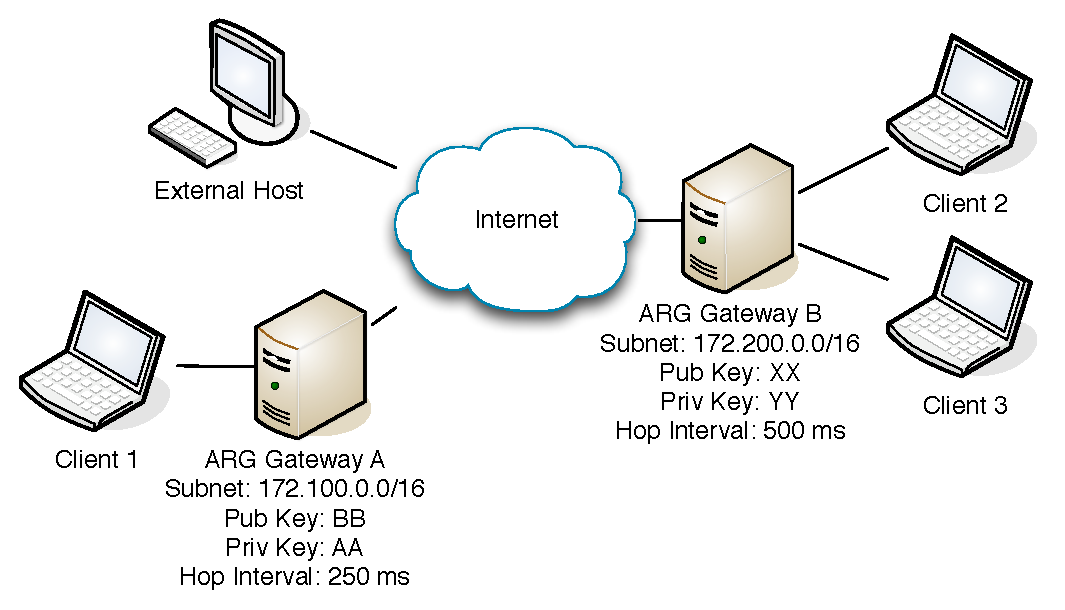
\includegraphics[width=1\textwidth]{arg_concept_network}
\end{frame}

\begin{frame}
	\frametitle{Background - Routing}
	Hierarchical nature of IP routing allows IP hopping to work
	\includegraphics<1>[width=1\textwidth]{routing_example_network}
	
	\begin{onlyenv}<2>
	\begin{table}
	\caption{IP routing example: Router A table}
	\centering
	\begin{tabular}{rccc}
	\toprule
	 & \textbf{IP} & \textbf{Mask} & \textbf{Interface}\\
	\hline
	1 & 10.5.0.25 & 255.255.0.0 & Port 1\\
	2 & 172.100.10.0 & 255.255.255.0 & Port 2\\
	3 & 172.100.0.0 & 255.255.0.0 & Port 3\\
	\bottomrule
	\end{tabular}
	\end{table}
	\end{onlyenv}
\end{frame}

\begin{frame}
	\frametitle{Goals}

\end{frame}

\section{Implementation}
\begin{frame}
	\frametitle{Implementation}

\end{frame}

\section{Methodology}
\begin{frame}
	\frametitle{Methodology}

\end{frame}

\section{Results}
\begin{frame}
	\frametitle{Results}

\end{frame}

\section{Conclusions}
\begin{frame}
	\frametitle{Conclusions}

\end{frame}

\section{Future Work}
\begin{frame}
	\frametitle{Future Work}

\end{frame}

\section{Summary}
\begin{frame}
	\frametitle{Summary}
	\tableofcontents
\end{frame}

\section{Questions}
\begin{frame}
	\frametitle{Questions}
	? \tbd{picture}
\end{frame}

%\section{Lessons Learned}
\begin{frame}
	\frametitle{Lessons Learned}
	Begin full pilot studies earlier
	\begin{itemize}
	\item Discover performance problems with results processing earlier
	\item See need to run more fine-grained hop intervals at higher end
	\end{itemize}
\end{frame}

\end{document}
